%!TEX TS-program = xelatex
%!TEX encoding = UTF-8 Unicode

\documentclass[%10pt,
			   a4paper,
			   twoside
			   ]{book}

\usepackage[T1]{fontenc}

\usepackage[margin=1in]{geometry}

\usepackage[parfill]{parskip}    % Activate to begin paragraphs with an empty line rather than an indent
\usepackage{graphicx}
\usepackage{amssymb}
\usepackage{wrapfig}
\usepackage{float} % they need to be placed in specific locations with the [H] (e.g. \begin{table}[H])

\usepackage{paralist}
\usepackage{array}
\usepackage{longtable}
\usepackage{multirow}

\usepackage{url}

\usepackage{multicol}
\usepackage{pdfpages}

\usepackage{tikz}
\usepackage{color}
\usepackage{lipsum}

%-------------------------------------------------------------
%----------------------------------------------------- FONTS -
%-------------------------------------------------------------

\linespread{1.04}

\usepackage{etoolbox}

\usepackage{fontspec,
			xltxtra,
			xunicode
			}

\defaultfontfeatures{Mapping=tex-text}

\setromanfont[Mapping=tex-text]{Alegreya}

\setsansfont[Scale=MatchLowercase,
			 Mapping=tex-text
			 ]{Fira Sans}

\setmonofont[]{Fira Mono}

\newfontfamily{\scaps}{Alegreya SC}

\newfontfamily\quotefont{Alegreya}
\AtBeginEnvironment{quote}{\quotefont\small}

\usepackage[italian,
			english
			]{babel}

\usepackage{lilyglyphs}

\usepackage[hang,
			small,
			labelfont=bf,
			up,
			textfont=it,
			up
			]{caption}

%-------------------------------------------------------------
%---------------------------------------------------- HEADER -
%-------------------------------------------------------------

\usepackage{fancyhdr}

\fancypagestyle{plain}{%
\fancyhf{} % clear all header and footer fields
%\fancyhead[CO,CE]{---Draft---}
\fancyfoot[RO,LE]{\fontsize{18pt}{18pt}\selectfont\thepage} % except the center
\renewcommand{\headrulewidth}{0pt}
\renewcommand{\footrulewidth}{0pt}}
\pagestyle{plain}

%-------------------------------------------------------------
%----------------------------------------------------- TITLE -
%-------------------------------------------------------------

\makeatletter
%\frameattext{<backgroundcolor>}{linecolor}{<linewidth>}
\newdimen\extraxsep
\newdimen\extraysep
\extraxsep=20mm
\extraysep=20mm
\newcommand\frameattext[3]{%
  \linethickness{#3}%
  \AddToShipoutPicture*{%
    \AtTextLowerLeft{%text-boder
       \put(\LenToUnit{-,5\extraxsep},\LenToUnit{-0.5\extraysep}){\color{#1}%
             \rule{\dimexpr\textwidth+\extraxsep\relax}{\dimexpr\textheight+\extraysep\relax}}%
       \put(\LenToUnit{-,5\extraxsep},\LenToUnit{-0.5\extraysep}){\color{#2}%
       \framebox(\LenToUnit{\dimexpr\textwidth+\extraxsep\relax},%
                 \LenToUnit{\dimexpr\textheight+\extraysep\relax}){}
       }
    }%
  }%
}
%\frameatpage{<backgroundcolor>}{linecolor}{<linewidth>}
\newcommand\frameatpage[3]{%
  \linethickness{#3}%
  \AddToShipoutPicture*{%
    \AtPageLowerLeft{%page-border
      \put(0,0){\color{#1}\rule{\paperwidth}{\paperheight}}%
      \put(\LenToUnit{\@wholewidth},\LenToUnit{\@wholewidth}){%
       \color{#2}\framebox(\LenToUnit{\dimexpr\paperwidth-2\@wholewidth\relax},%
                  \LenToUnit{\dimexpr\paperheight-2\@wholewidth\relax}){}%
      }%
    }%
  }%
}

\makeatother

%-------------------------------------------------------------
%-------------------------------------------------- DOCUMENT -
%-------------------------------------------------------------

\begin{document}

\setlength{\columnsep}{.4in}

\frameattext{white}{black}{2pt}

\begin{center}
	~
	\vfill
	
    \fontsize{19}{19}\selectfont{Giuseppe SILVI}
    	\vspace{.3in}
		\noindent\makebox[\linewidth]{\rule{.3\paperwidth}{1pt}}
	\fontsize{51}{51}\selectfont{\emph{l'invito all'ascolto}} \\
		\vfill %\vspace{1in}	
		~
		\vfill
		
    \fontsize{19}{19}\selectfont{COME/01 \\ esecuzione ed interpretazione della \\musica elettroacustica \\ 2016/2017} \\
							     
		\vfill
	\fontsize{19}{19}\selectfont{draft 002\\ \today}
	
	\vfill
	~

\end{center}
%\maketitle

\thispagestyle{empty}

%\clearpage
%
%\thispagestyle{empty}
%
%~
%
%\clearpage
%
%\tableofcontents
%
%~\vfill
%
%
\includegraphics[width=.25\columnwidth]{images/by-nc-sa}\\
%\emph{A. Sax.} by Giuseppe Silvi is licensed under a Creative Commons \\
%Attribution-NonCommercial-ShareAlike 4.0 International License.\\
%Permissions beyond the scope of this license may be available at\\
%giuseppesilvi.com/asax.%\marginpar{prova} 
%
%
\clearpage
\thispagestyle{empty}

Conservatorio di Musica S. Cecilia di Roma \\
DIPARTIMENTO DI MUSICA ELETTRONICA \\
Esecuzione ed Interpretazione della Musica Elettronica - COME/01 \\
Anno accademico 2016/2017
\vfill

inserire licenza uso

\clearpage

\tableofcontents

\clearpage

\thispagestyle{empty}

\includepdf[scale=1.05,
		    pagecommand={
		    	\begin{tikzpicture}[
					remember picture,
					overlay]
		    	\node [xshift=2cm,yshift=1cm] at (current page.south west) {\color{white}{\emph{Roberto \textbf{Masotti}}}};
				\end{tikzpicture}}
		    ]{masotti/cage.pdf}
		    
%-------------------------------------------------------------
%------------------------------- JOHN CAGE - CARTRIDGE MUSIC -
%-------------------------------------------------------------

\chapter*{John Cage.\\\emph{Cartridge Music}. 1960}
\addcontentsline{toc}{chapter}{John Cage. \emph{Cartridge Music}. 1960}

	\begin{flushright}
		\textit{Nella nostra anima c'\`e una incrinatura che, se sfiorata, \\
		risuona come un vaso prezioso riemerso dalle profondit\`a della terra} \\
		Wassilly Kandinsky - \emph{Lo Spirituale nell'Arte}
	\end{flushright}

	\begin{flushright}
		\textit{Music of Changes // John ChAnGEs} \\
		Pierre Boulez
	\end{flushright}

	\begin{flushright}
		\textit{Si dice che i compositori abbiano orecchio per la musica e \\
		di solito significa che non sentono nulla che arrivi alle loro orecchie. \\
		Le loro orecchie sono murate dai suoni di loro creazione.} \\
		John Cage - \emph{45' for a Speaker} (1954)
	\end{flushright}

\bigskip

\begin{multicols}{2}

\begin{quote}
	Ogni opera d'arte \`e figlia del suo tempo, e spesso \`e madre dei nostri
	sentimenti.
	
	Analogamente, ogni periodo culturale esprime una sua arte, che non si ripeter\`a mai pi\`u.
	Lo stesso sforzo di ridar vita a principi estetici del passato pu\`o creare al massimo delle opere d'arte che sembrano bambini nati morti.
	Noi non possiamo, ad esempio, avere la sensibilit\`a e la vita interiore\footnote{Wassilly Kandinsky, \emph{Lo Spirituale nell'Arte}, SE. 1989}\ldots
\end{quote}

di John Cage, in luogo degli antichi Greci, come avrebbe continuato Kandinsky.
Ci deve essere un certo grado di consapevolezza in relazione al livello di
comprensione-incomprensione del pensiero di John Cage. Ma ammettendo di
averlo compreso, per quanto noi potremmo approfondire lo studio del suo
pensiero e della sua musica, potremmo solo arrivare ad imitarne alcuni tratti
stilistici. E se tentassimo di

\begin{quote}
	adottare i loro princ\`{\i}pi, non faremmo che produrre forme simili alle loro, ma prive di anima\footnote{\emph{idem}}.
\end{quote}

Questo non esclude che si possa riuscire ad entrare in contatto con le
motivazioni e gli stimoli artistici, soprattutto
e si attinge ai tratti
condivisi tra le somiglianze delle forme artistiche,

\begin{quote}
	delle aspirazioni interiori e degli ideali (che un tempo erano stati raggiunti
	e poi vennero dimenticati), la somiglianza cio\`e fra i climi culturali di due
	epoche che pu\`o portare alla ripresa di forme che erano gi\`a state utilizzate in
	passato per esprimere le stesse tensioni\footnote{\emph{idem}}.
\end{quote}

Costruire il repertorio, utilizzare il tempo presente per reinventare il tempo passato.
Respirare la stessa aria di un autore non pi\`u presente attraverso la comprensione, intima,
a livello percettivo, delle molteplici ineffabilit\`a della sua epoca.
Consumare la sua poetica acquisendo ogni io sotteso e nascosto. Percepirne il dopo,
il passato meno passato delle conseguenze lasciate al mondo, al suo futuro.
Tutto questo, di un personaggio complesso ed enorme come John Cage, \`e piuttosto complesso.

%John Cage \`e stato al mondo in maniera totale.

Essere John Cage, \emph{compositore}: ha scritto testi, libri, ha tenuto conferenze, ha dipinto,
ha consultato gli oracoli, ha meditato, ha suonato, ha indagato, ha scritto musica.

%Questo essere, di una sensibilit\`a totale, significa utilizzare la percezione attraverso tutti i canali percettivi di cui si \`e dotati.

In questo senso l'attivit\`a artistica, plastica, sonora, letteraria \`e manifestazione di uno
stesso percepire comune.

\begin{quote}
	\emph{Geometria}
	
	Dentro ogni forma, dietro ogni figura si nasconde una geometria. Questo nascondersi \`e come
	un silenzio che filtra alla superficie con linee sottili e rende intellegibili le forme
	senza che sia necessario comprenderle a fondo: \`e proprio tale muta eloquenza a comunicare
	allo sguardo il senso intimo di un'opera.
	
	La geometria ha in s\'e elementi ineffabili, pur se immersa in visioni corrusche, in cosmi
	travolti dalle dissimmetrie o capovolti in spirali avvolgenti; e non \`e soltanto
	l'austera evidenza ortogonale di una struttura a farsi Geometria, ma una risonanza segreta
	a far brillare e fiammeggiare, a sollevare e sospendere, ad affermare o togliere al
	corpo della pittura il suo \emph{necessario} silenzio.
\end{quote}

Tra le caratteristiche non convenzionali di John Cage ce n'\`e per me una piuttosto
curiosa: davanti ad una mastodontica produzione musicale, ad una quasi totale
assenza di apparato critico strutturato, non \`e difficile individuare gli
\emph{stili musicali} di John Cage, dividendoli in quattro sezioni temporali
scandite da date piuttosto precise: 1939, 1951, 1969.

Le prime opere sono caratterizzate da un cromatismo strutturato e dalla
sperimentazione soprattutto con gli strumenti a percussione.
Con \emph{Firts Construction in Metal} del 1939 realizza la prima opera
utilizzando strutture temporali. Nel 1951 con \emph{Music of Changes} e
\emph{Imaginary Landscape No. 4} si compie il passaggio dall'organizzazione
sistematica alla combinazione di elementi sistematici, gusti personali e
indeterminazione casuale. Gli anni che seguirono il 1951 furono decisivi per
lo sviluppo delle operazioni casuali.

\`e dal 1957 che Cage inizi\`o a concepire opere nelle quali tutti gli aspetti
dell'interpretazione fossero indeterminati. Tutte le decisioni in merito ai
suoni e alla loro successione sono delegate dal compositore all'esecutore;
la partitura permette soltanto di assicurare una certa disciplina quanto al
modo di porendere devisioni che produrranno dei risultati imprevedibili. In quegli
anni \emph{Fontana Mix, Cartridge Music}\footnote{\emph{Cartridge
Music} at John Cage's Database of Works www.johncage.org: \\ This work was later used as music for the choreographed piece by Merce Cunningham
entitled Changing Steps, with stage and costume design by Charles Atlas (from 1973,
Mark Lancaster); still later, it was used for the choreographed pieces by
Cunningham entitled Exercise Piece II and Exercise Piece III.
The word 'Cartridge' in the title refers to the cartridge of phonographic
pick-ups, into the aperture of which is fitted a needle. In Cartridge Music,
the performer is instructed to insert all manner of unspecified small objects
into the cartridge; prior performances have involved such items as pipe cleaners,
matches, feathers, wires, etc. Furniture may be used as well, amplified via
contact microphones. All sounds are to be amplified and are controlled by the
performer(s). The number of performers should be at least that of the cartridges,
but not greater than twice the number of cartridges. Each performer makes his or
her own part from the materials provided: 20 numbered sheets with irregular
shapes (the number of shapes corresponding to the number of the sheet) and 4
transparencies, one with points, one with circles, another with a circle marked
like a stopwatch, and the last with a dotted curving line, with a circle at one
end. These transparencies are to be superimposed on one of the 20 sheets, in
order to create a constellation from which one creates one's part. It is also
possible to create other pieces from these materials, such as Duet for Cymbal
or a Piano Duet. Cage also used Cartridge Music as a means to compose several
of his lectures, including ?Where Are We Going? And What Are We Doing?? (1960),
?Rhythm, Etc.? (1962), ?Jasper Johns: Stories and Ideas? (1963), and
?On Robert Rauschenberg, Artist, and His Work? (1961).} e la serie delle \emph{Variations},
consisteva in fogli lucidi trasparenti, con linee, punti e curve, a partire dalle
quali si costruivano partiture (strutture, materiali e relazioni, applicabili non
solo alla musica) che era possibile eseguire in diverse circostanze.

La regolarit\`a e la continuit\`a estetica di questa produzione fu interrotta nel 1969
con il brano \emph{HPSCHD} per sette clavicembali amplificati e tape multicanale.
La musica di Cage ri riappropria quindi di una notazione convenzionale in uninione
con la tecnicna del \emph{collage}. L'anno successivo Cage porse le prime domande
di composizione all'\emph{I Ching}.

\begin{quote}
	I procedimenti casuali sono solo uno strumento tra altri che Cage ha utilizzato
	per perseguire coerentemente un unico scopo: l'accettazione disciplinata, in
	contesti musicali, di ci\`o che fino ad allora era stato rifiutato. �Sono sempre
	stato dalla parte delle cose che non si devono fare�, ha osservato una volta,
	�cercando il modo di rimettere in gioco gli elementi rifiutati�\footnote{William
	Brooks, \emph{Scelte e Cambiamenti Nella Musica Recente di Cage} 1982}.
\end{quote}

\centering{***}

\begin{quote}
	L'artista cercher\`a di suscitare sentimenti pi\`u delicati, senza nome [\ldots]
	Attualmente per\`o lo spettatore \`e quasi sempre incapace di emozioni.
	Nell'opera d'arte cerca una mera imitazione della natura a scopo pratico.
	[\ldots] certo l'immedesimazione (e la contrapposizione) non deve essere
	vacua o superficiale: anzi, l'atmosfera dell'opera deve rendere pi\`u
	coinvolgente e visionaria l'atmosfera in cui \`e immerso lo spettatore. [\ldots]
	L'affinamento e la diffusione della loro voce nel tempo e nello spazio
	rimangono per\`o un fatto soggettivo, che non esaurisce le potenzialit\`a dell'arte.
\end{quote}

\begin{quote}
	Indeterminacy gets personal preference out of the compositional process.\footnote{Alvin Lucier, Music 109}
\end{quote}

\begin{quote}
    Cage claimed to be an anarchist. By that he didn't mean that everyone simply does whatever they want to or does things in a shoddy manner. If everybody did whatever they did as well as they could, there wouldn't be the need to refer to a higher authority.	
\end{quote}

\begin{quote}
	He wanted to make a composition that was free of personal taste and memory, which existed outside the traditions of music, and was, above all, free of psychology.
There are wonderful images in the \emph{I Ching}? Fire in the Lake, The Wanderer, Inner Truth? but Cage didn't use them. 
\end{quote}

\begin{quote}
	La situazione diventava abbastanza confusa, con le persone che ruotavano diverse manopole, senza poter in alcun modo prevedere il risultato delle proprie azioni. (Tom Darter 1982. Lettera a uno sconosciuto)
\end{quote}

\begin{quote}
	\emph{Cartridge Music} prevede che ci siano numerose persone che eseguono programmi che hanno determinato per mezzo di materiali. Ma le azioni di una persona modificheranno in modo non intenzionale le azioni di un'altra, dal momento che le azioni prevedono dei cambiamenti nei controlli di tono e di volume. Cos\`i ci si \`o trovare a suonare qualcosa senza ottenere alcun suono. (Cole Gagne e Tracy Caras 1982)
\end{quote} 

\begin{quote}
	\ldots utilizza l'elettronica, ma fa uso anche di oggetti di scarto che sono parte integrante della nostra esistenza quotidiana. Abbiamo una situazione complessa [\ldots] e degli oggetti a cui sono applicati dei \emph{pick-up} [\ldots] Si entra in una situazione simile a quando si imbocca il lungo tunnel del New Jersey. [\ldots] Una persona pu� magari abbassare il volume, mentre qualcun altro sta suonando qualcosa. Cause ed effetti sono scollegati. Gli elementi personali sembrano far s� che il meccanismo non funzioni in modo proprio perfetto.
\end{quote} 

Rapporto con il concerto e la sala da concerto

\begin{quote}
	Se c'� un concerto come questo il pubblico � in grado di sentire anche quando esce dalla sala, e i rumori non sembreranno loro cos� spiacevoli come avevano pensato. [\ldots] � un tentativo di apriore le nostre menti a possibilit� diverse da quelle che possiamo ricordare, e che gi� sappiamo che ci piacciono. Si deve far qualcosa che ci liberi dai nostri ricordi, dalle nostre preferenze. (David Sterrit 1982)
\end{quote} 

\begin{quote}
	\emph{L'atto di formulare domande rappresenta, di fatto, un processo creativo}.\\
	� proprio quello di c ui sono convinto.\\
	\emph{\emph{Cartridge Music} costituisce un buon esempio. in qualche modo � possibile affermare che \emph{Cartridge Music} sempre come \emph{Cartridge Music}. Quel pezzo manterr� la sua identit� anche se da un evento all'altro potranno accadere molte cose diverse, e questo a causa dell'invenzione originaria del mezzo attraverso il quale i suoni operano, cio� le testine magnetiche stesse. Questo potrebbe consentirci di affermare che, in una certa misura, ciascun pezzo di John Cage suoner� sempre sia come qualcosa in s� che come un pezzo di John Cage. Pensa questo sia vero?} \\
	Parzialmente.
	\emph{Fino a che punto non � vero?}
	Be, mi fa sempre piacere ricordare quanto avvenne a Beverly Hills mentre prendevo un drink con un'amica, di cui ho dimenticato il nome. Mentre Stavamo parlando e bevendo, c'era un disco che suonava in un'altra stanza, e mi colp� perch� si trattava di un pezzo molto interessante. Le chiesi cosa fosse e lei rispose: <<Non stai parlando sul serio vero?>>. Si trattava di un mio pezzo, e non lo avevo affatto riconosciuto.\\
	\emph{E scopr� di che pezzo si trattava?}\\
	Era proprio \emph{Cartridge Music}. Quando david Tudor ed io lo registrammo per la Mainstream, l'etichetta discografica di Earle Brown, Earle ci chiese se desideravamo ascoltare il missaggio finale, e tutti e due rispondemmo che non volevamo sentirlo, e cos� quella fu probabilmente la prima volta che lo ascoltai. (Tom Darter 1982)
	
\end{quote} 




\end{multicols}


\clearpage

\thispagestyle{empty}

\includepdf[scale=1.03,
		    pagecommand={
		    	\begin{tikzpicture}[
					remember picture,
					overlay]
		    	\node [xshift=2cm,yshift=1cm] at (current page.south west) {\color{white}{\emph{Heinz \textbf{Karnine}}}};
				\end{tikzpicture}}
		    ]{stockhausen/stockhausen.pdf}
		    
%-------------------------------------------------------------
%---------------------------- KARLHEINZ STOCKHAUSEN - MANTRA -
%-------------------------------------------------------------

\chapter*{Karlheinz Stockhausen.\\\emph{Mantra}. 1970}
\addcontentsline{toc}{chapter}{Karlheinz Stockhausen. \emph{Mantra}. 1970}

	\begin{flushright}
		\textit{Nella nostra anima c'� una incrinatura che, se sfiorata, \\
		risuona come un vaso prezioso riemerso dalle profondit� della terra} \\
		Wassilly Kandinsky - \emph{Lo Spirituale nell'Arte}
	\end{flushright}

	\begin{flushright}
		\textit{Music of Changes // John ChAnGEs} \\
		Pierre Boulez
	\end{flushright}

	\begin{flushright}
		\textit{Si dice che i compositori abbiano orecchio per la musica e \\
		di solito significa che non sentono nulla che arrivi alle loro orecchie. \\
		Le loro orecchie sono murate dai suoni di loro creazione.} \\
		John Cage - \emph{45' for a Speaker} (1954)
	\end{flushright}

\bigskip

\begin{multicols}{2}
1969 quattro persone che chiacchierano di questo e quello in una macchina tra medicine connecticut e boston.
lungo la strada scrive su una busta che aveva in tasca una melodia che contiene tutte e dodici le note. un anno dopo
inizia il suo lavoro per due pianoforti e riprende questa melodia.
tutta la melodia stirata sull'intera durata del brano, un'ora. e contemporanemamente compressa nella pi� piccola portzione temporale.
ogni nota a sua volta richiamava a se tutte le altre note rendendo per ognuno di questi punti il complesso delle 12 note. Il tutto somiglia
molto ad un sistema di stelle.

tutta la melodia � il mantra, come fosse una formula. ci sono 4 regioni separate da pause. la prima regione � formata da 4 note. la seconda da 2. la terza da 5 la quarta da 3

mirror

spiegher� come il mantra, la formula, pu� essere usata per l'intera composizione, per fare questo ho bisogno della variazione

trovare qualcosa sulle lezioni inglesi?

dobbiamo immaginare come se ogni nota determina un'intera sezione di una certa composizione

combinare le sezioni tra loro con la tecnica delle variazioni

non ho costruito la formula sulla base di una scala cromatica 

\end{multicols}


\begin{table}[htp]
\caption{Melodia - Formula - Regioni}
\begin{center}
\begin{sf}{\footnotesize
\begin{tabular}{r c c c c c c c c c c c c c c c c c c }

       \textbf{altezze} & \multicolumn{4}{c}{4} 	 & \multirow{3}*{pausa 3} & \multicolumn{3}{c}{2} & \multirow{3}*{pausa 2} & \multicolumn{5}{c}{5}  & \multirow{3}*{pausa 1} & \multicolumn{3}{c}{3}  \\
\textbf{durata regione} & \multicolumn{4}{c}{10} &                        & \multicolumn{3}{c}{6} &                        & \multicolumn{5}{c}{15} &                        & \multicolumn{3}{c}{12}   \\
  \textbf{suddivisione} & 1 & 2 & 3 & 4          &                        & 2 & 2 & 2             &                        & 5 & 2 & 1 & 3 & 4      &                        & 4 & 2 & 6 \\

\end{tabular}}
\end{sf}
\end{center}
\label{default}
\end{table}%

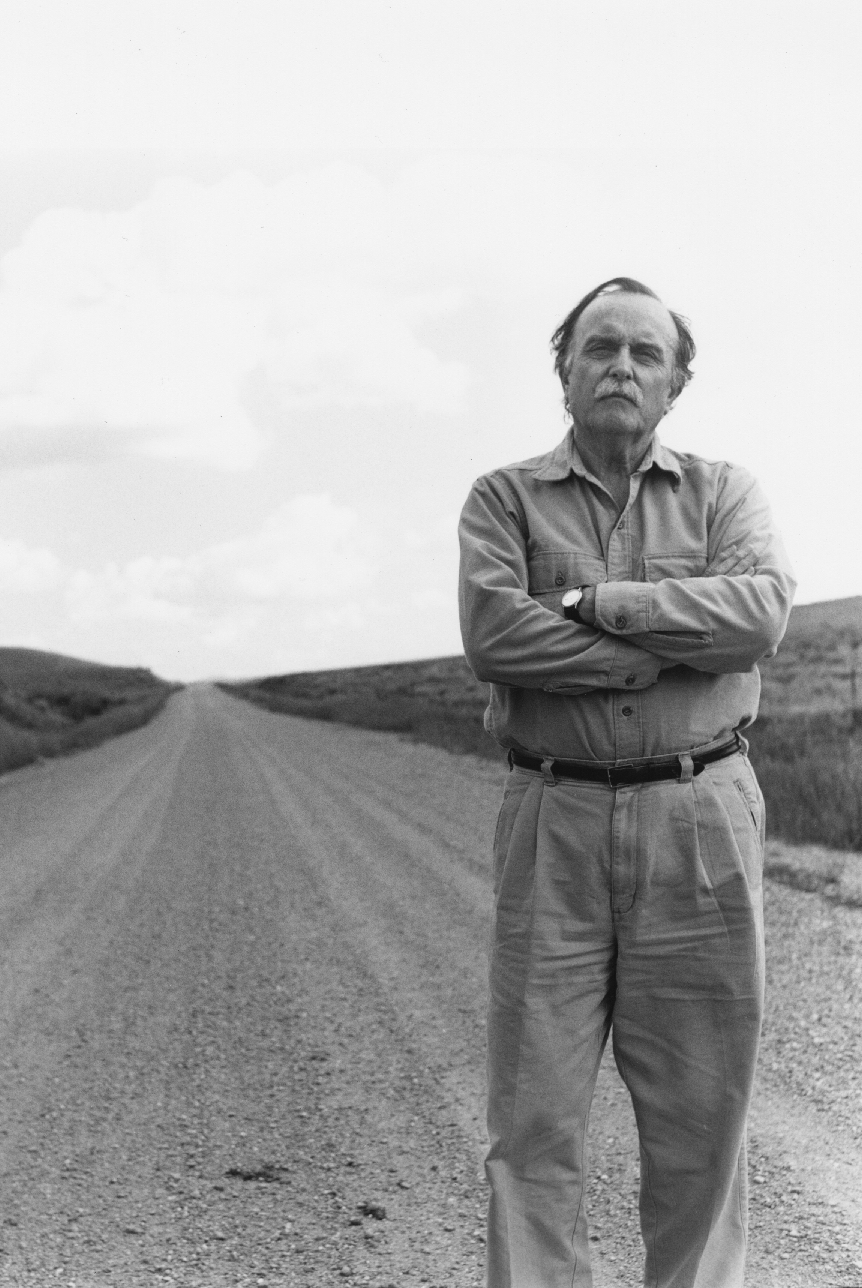
\includepdf[scale=1.1]{lucier/lucier_road_cc.pdf}

%-------------------------------------------------------------
%------------------------------- ALVIN LUCIER - EVER PRESENT -
%-------------------------------------------------------------

\chapter*{Alvin Lucier. \\
			\emph{Waves Song}. 1998\\
			\emph{Ever Present}. 2002}
\addcontentsline{toc}{chapter}{Alvin Lucier. \emph{Waves Song}. 1998 -- Ever Present. 2002}

	\begin{flushright}
		\textit{Nella nostra anima c'� una incrinatura che, se sfiorata, \\
		risuona come un vaso prezioso riemerso dalle profondit� della terra} \\
		Wassilly Kandinsky - \emph{Lo Spirituale nell'Arte}
	\end{flushright}

	\begin{flushright}
		\textit{Music of Changes // John ChAnGEs} \\
		Pierre Boulez
	\end{flushright}

	\begin{flushright}
		\textit{Si dice che i compositori abbiano orecchio per la musica e \\
		di solito significa che non sentono nulla che arrivi alle loro orecchie. \\
		Le loro orecchie sono murate dai suoni di loro creazione.} \\
		John Cage - \emph{45' for a Speaker} (1954)
	\end{flushright}

\bigskip

\begin{multicols}{2}

\begin{quote}
	On 24 September 1960, I attended a concert by John Cage, David Tudor, Merce Cunningham and Carolyn Brown at La
	Fenice Theater in Venice. I had come to Venice that summer on a Fulbright Scholarship to study at the Benedetto
	Marcello Conservatory before going on to Rome where I would spent the next 2 years. The Cage-Tudor event came
	like a bolt out of the blue-all the protocols of the concert situation were violated.
	The concert began, as I remember, with David Tudor striding down the aisle of the theatre and diving under 
	the piano, hitting the underside to make the first sound of the concert. Cage made an appearance playing
	a piano that rose up into the pit hydraulically. The four per- formers had cards upon which were written instructions
	regarding sound s or actions to be made and where to make them. The entire theatre was used-stage, aisles, balconies.
	The work was \emph{Music Walk with Dancers} (1958). During that concert a man walked down the aisle and struck the piano
	with an umbrella and announced: "Now I am composer!" At the height of the pandemonium, Cage was tuning a radio 
	that he used as a sound source, and the Pope came on asking for peace on earth.	
	
	That concert forever altered the way I thought about mu- sic. Until that time I had followed the conventional pattern of
	composer-performer-audience relationships. One would compose a work, wait for some soloist, ensemble or orchestra to perform it, then hope that the audience would like it. It was a lonely life; a waiting game. 
\end{quote}

di John Cage, in luogo degli antichi Greci, come avrebbe continuato Kandinsky.
Ci deve essere un certo grado di consapevolezza in relazione al livello di
comprensione-incomprensione del pensiero di John Cage. Ma ammettendo di
averlo compreso, per quanto noi potremmo approfondire lo studio del suo
pensiero e della sua musica, potremmo solo arrivare ad imitarne alcuni tratti
stilistici. E se tentassimo di


\end{multicols}

\clearpage

\thispagestyle{empty}

\includepdf[offset=80 0,
			scale=2.2,
		    pagecommand={
		    	\begin{tikzpicture}[
					remember picture,
					overlay]
		    	\node [xshift=2cm,yshift=1cm] at (current page.south west) {\color{white}{\emph{Kai \textbf{Bienart}}}};
				\end{tikzpicture}}
		    ]{discipio/SCIP030BN.pdf}
		    
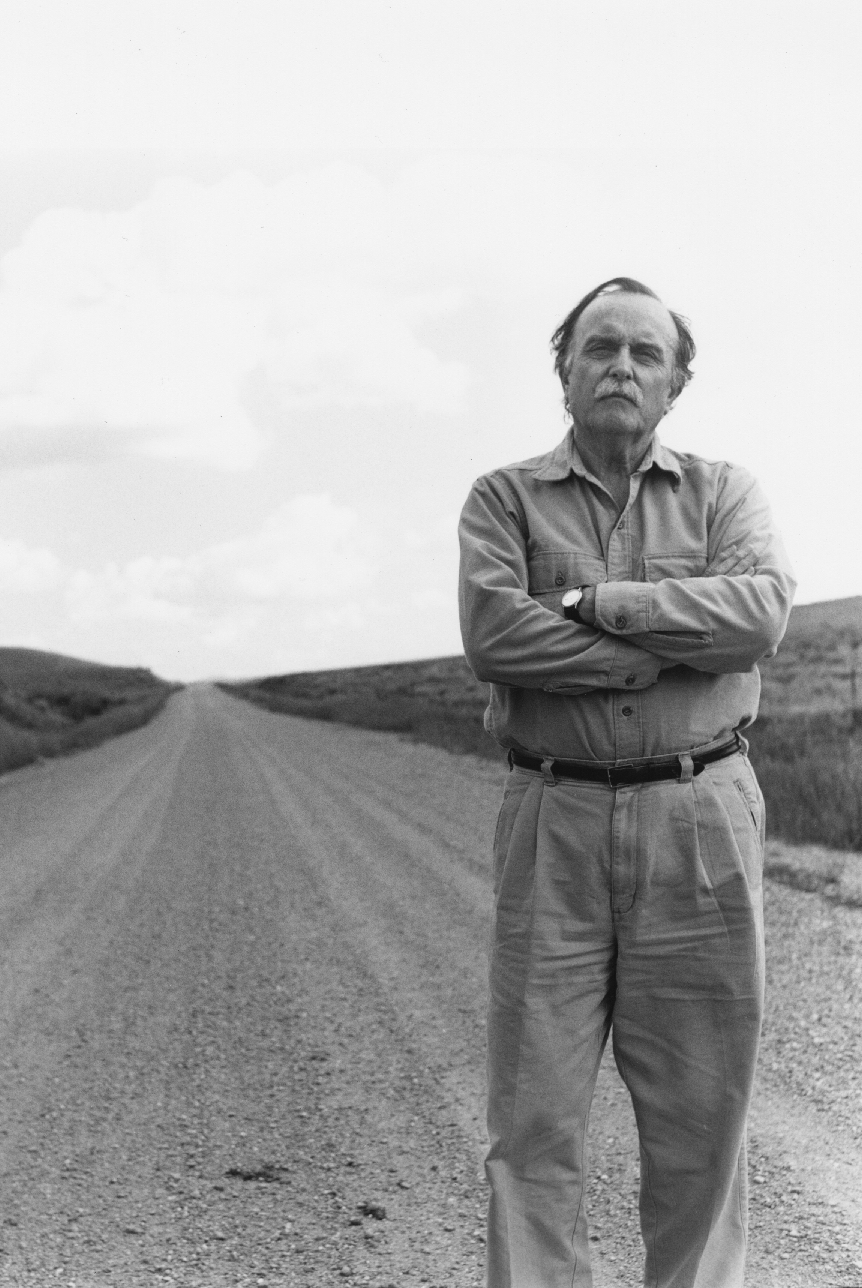
\includepdf[scale=1.1]{lucier/lucier_road_cc.pdf}

%-------------------------------------------------------------
%------------------------------- ALVIN LUCIER - EVER PRESENT -
%-------------------------------------------------------------

\chapter*{Agostino di Scipio. \emph{Audible Ecosystemic 2A}. 2003}
\addcontentsline{toc}{chapter}{Agostino di Scipio. \emph{Audible Ecosystemic 2A}. 2003}

	\begin{flushright}
		\textit{Nella nostra anima c'� una incrinatura che, se sfiorata, \\
		risuona come un vaso prezioso riemerso dalle profondit� della terra} \\
		Wassilly Kandinsky - \emph{Lo Spirituale nell'Arte}
	\end{flushright}

	\begin{flushright}
		\textit{Music of Changes // John ChAnGEs} \\
		Pierre Boulez
	\end{flushright}

	\begin{flushright}
		\textit{Si dice che i compositori abbiano orecchio per la musica e \\
		di solito significa che non sentono nulla che arrivi alle loro orecchie. \\
		Le loro orecchie sono murate dai suoni di loro creazione.} \\
		John Cage - \emph{45' for a Speaker} (1954)
	\end{flushright}

\bigskip

\begin{multicols}{2}

\begin{quote}
	On 24 September 1960, I attended a concert by John Cage, David Tudor, Merce Cunningham and Carolyn Brown at La
	Fenice Theater in Venice. I had come to Venice that summer on a Fulbright Scholarship to study at the Benedetto
	Marcello Conservatory before going on to Rome where I would spent the next 2 years. The Cage-Tudor event came
	like a bolt out of the blue-all the protocols of the concert situation were violated.
	The concert began, as I remember, with David Tudor striding down the aisle of the theatre and diving under 
	the piano, hitting the underside to make the first sound of the concert. Cage made an appearance playing
	a piano that rose up into the pit hydraulically. The four per- formers had cards upon which were written instructions
	regarding sound s or actions to be made and where to make them. The entire theatre was used-stage, aisles, balconies.
	The work was \emph{Music Walk with Dancers} (1958). During that concert a man walked down the aisle and struck the piano
	with an umbrella and announced: "Now I am composer!" At the height of the pandemonium, Cage was tuning a radio 
	that he used as a sound source, and the Pope came on asking for peace on earth.	
	
	That concert forever altered the way I thought about mu- sic. Until that time I had followed the conventional pattern of
	composer-performer-audience relationships. One would compose a work, wait for some soloist, ensemble or orchestra to perform it, then hope that the audience would like it. It was a lonely life; a waiting game. 
\end{quote}

di John Cage, in luogo degli antichi Greci, come avrebbe continuato Kandinsky.
Ci deve essere un certo grado di consapevolezza in relazione al livello di
comprensione-incomprensione del pensiero di John Cage. Ma ammettendo di
averlo compreso, per quanto noi potremmo approfondire lo studio del suo
pensiero e della sua musica, potremmo solo arrivare ad imitarne alcuni tratti
stilistici. E se tentassimo di


\end{multicols}

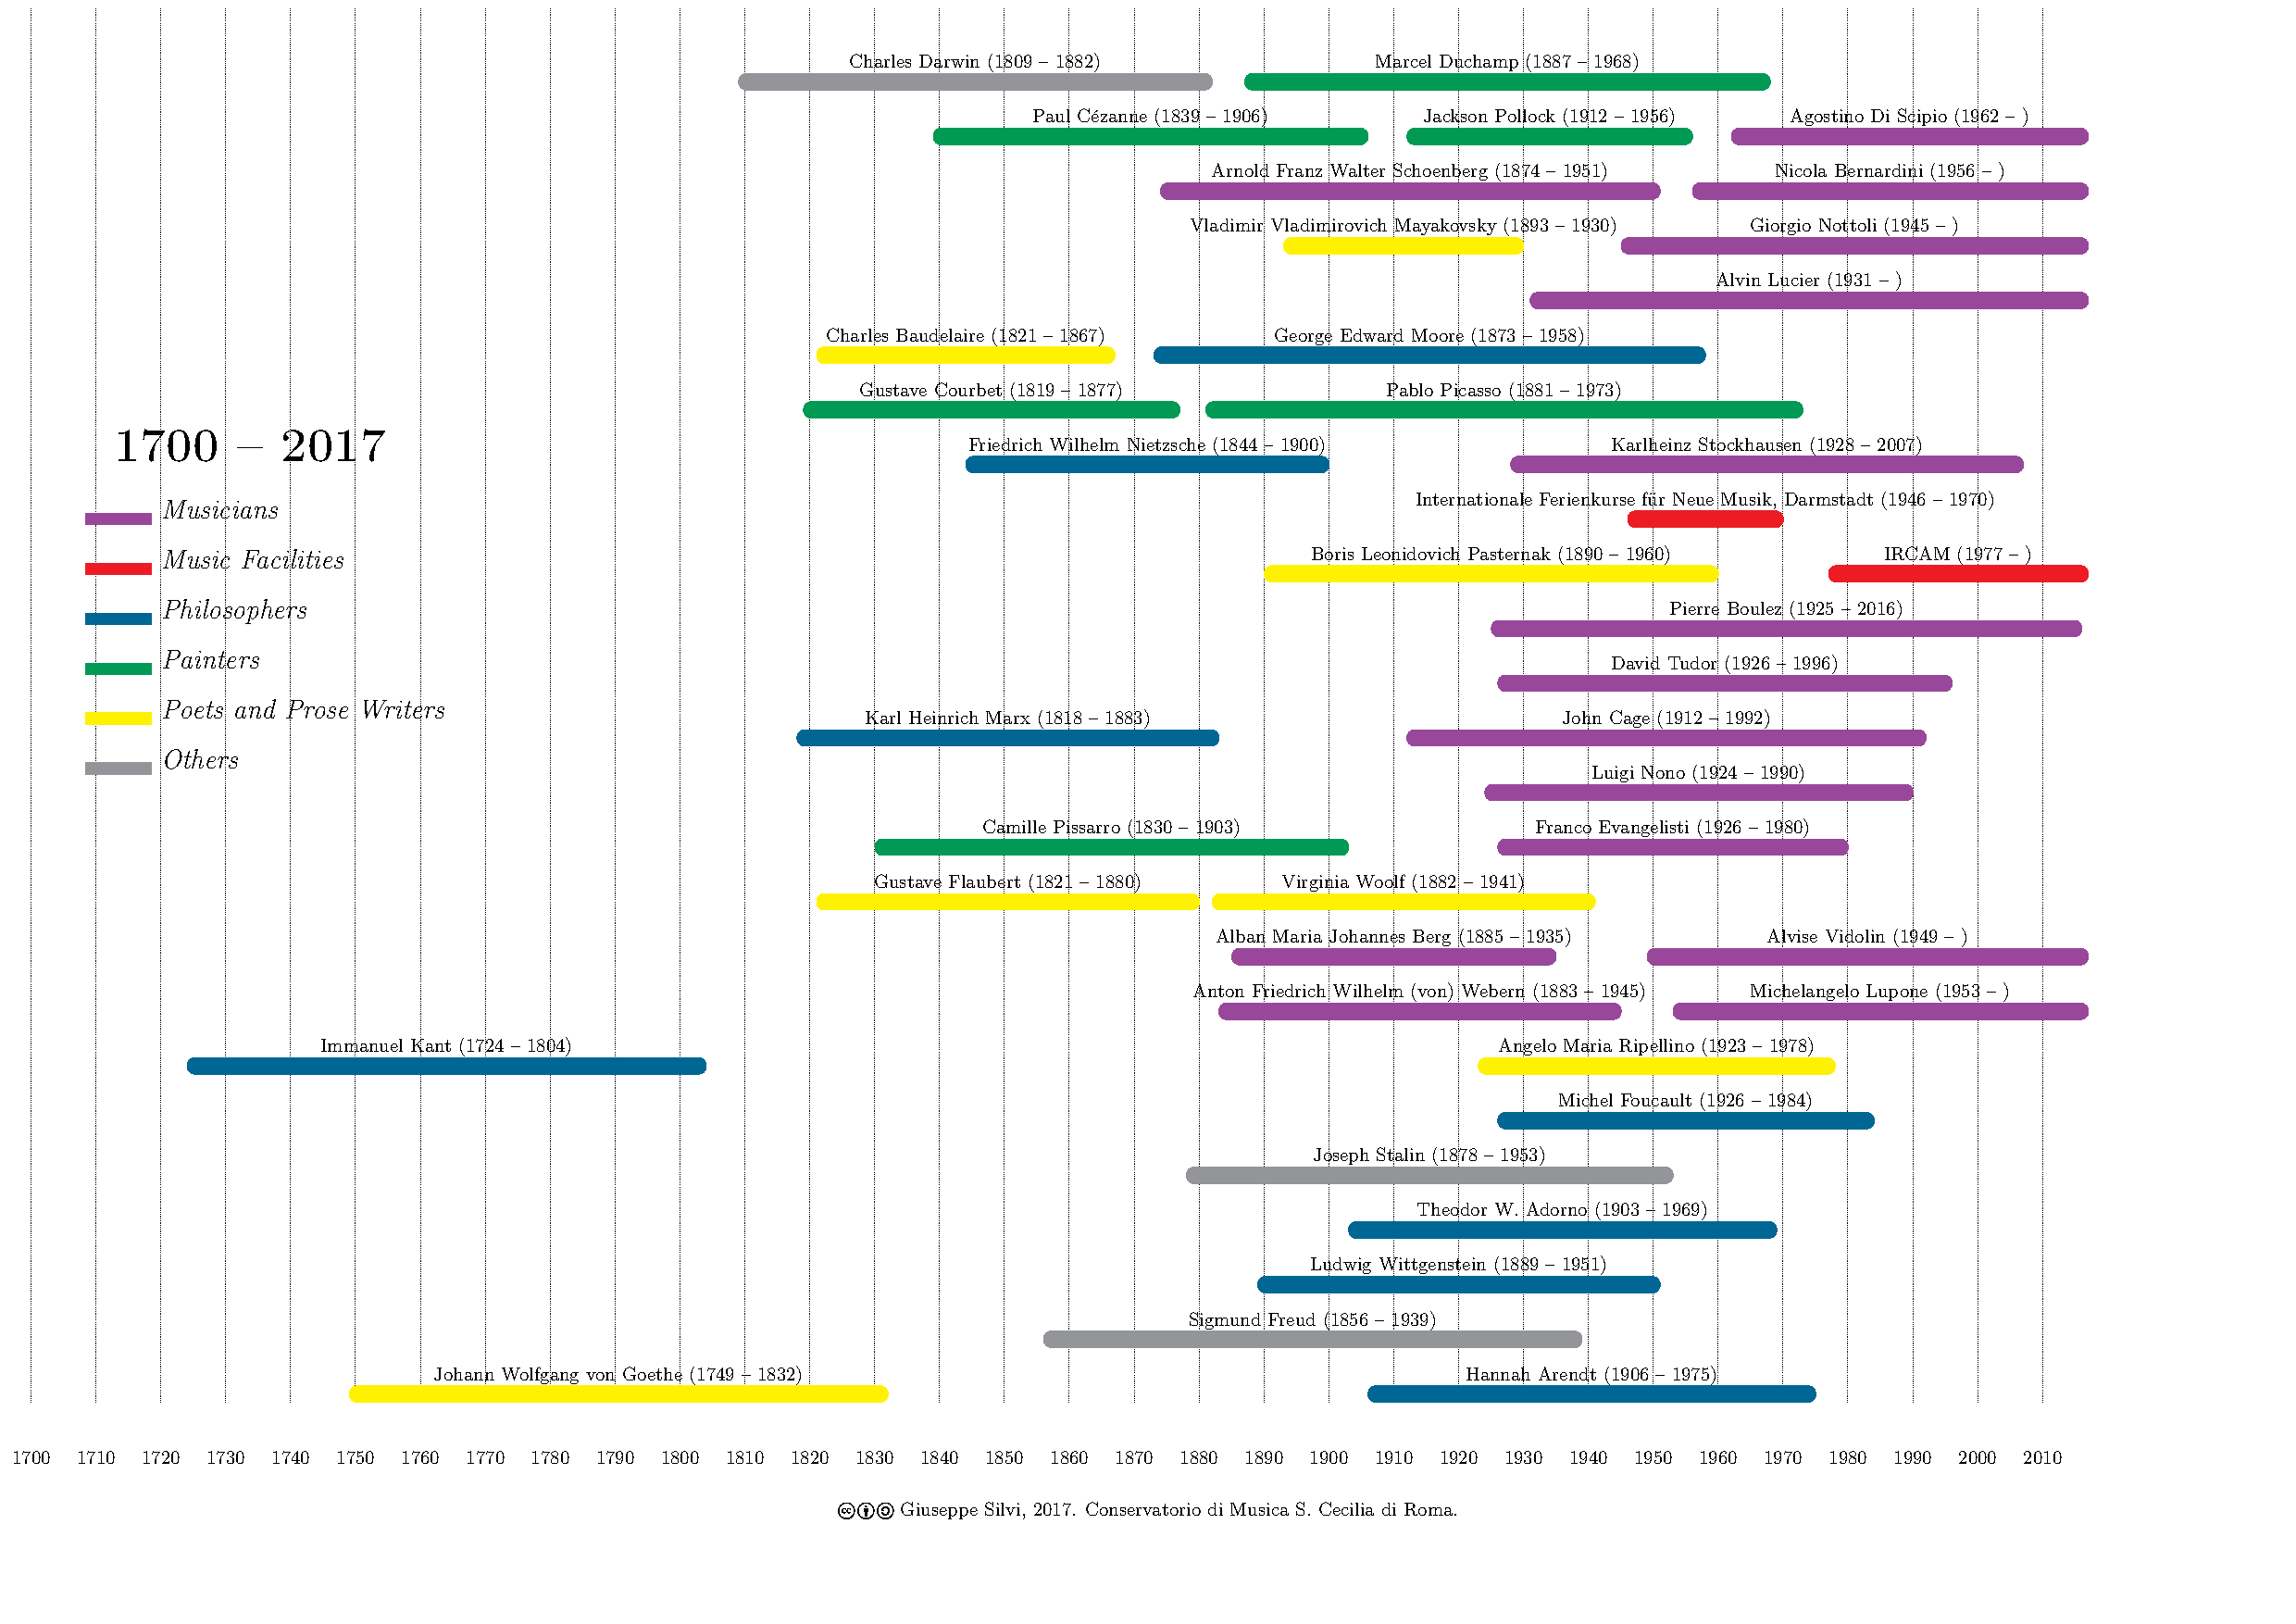
\includepdf[rotate=90]{_timeline/cosmologia.pdf}

%\begin{figure}[htbp]
%\begin{center}
%\includegraphics[width=.99\textwidth]{../../../Photos/090415_capolona.JPG}
%\caption*{S.T.ONE \& S.T.ON3S - Centro Ricerche Musicali, Rome - July 2015, 17th}
%\label{default}
%\end{center}
%\end{figure}

\end{document}
